\normaltrue \difficilefalse \tdifficilefalse
\correctionfalse
%\UPSTIidClasse{11} % 11 sup, 12 spé
%\newcommand{\UPSTIidClasse}{11}

\exer{Roburoc $\star$ \label{C2:04:68}}
%% CCMP 2009
\setcounter{numques}{0}
\UPSTIcompetence[2]{C2-04}
\index{Compétence C2-04}
\index{Correcteur}
\index{Correcteur proportionnel intégral}
\index{Roburoc}


\ifcorrection
\else
\textbf{Pas de corrigé pour cet exercice.}
\fi

\ifprof
\else

Soit le schéma-blocs suivant. 

\begin{center}
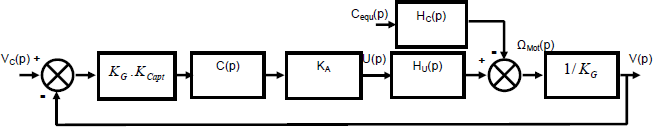
\includegraphics[width=\linewidth]{68_01}
\end{center}

On a $H_U(p) = \dfrac{K_U}{\left( T_1 p +1 \right)\left( T_2 p +1 \right)}$ et $H_C(p) = \dfrac{K_C \left( 1+\dfrac{L}{r}p\right)}{\left( T_1 p +1 \right)\left( T_2 p +1 \right)}$. $K_U =\SI{8,3}{rad.s^{-1}.V^{-1}}$, $K_C = \SI{152,7}{rad.s^{-1}.N^{-1}.m^{-1}}$, $T_1 = \SI{2,1}{ms}$ et $T_2 = \SI{0,36}{ms}$.

\textbf{Etude des performances sans correction : $C( p) =1$}

Nous distinguerons dans la suite :
\begin{itemize}
\item l’étude en poursuite : le couple de perturbation équivalent $C_{\text{equ}} (t)$ est nul. $V_c(t)$ varie ;
\item l’étude en régulation : la vitesse de consigne de la plate-forme $V_c(t)$  est nulle. $C_{\text{equ}} (t)$ varie.
\end{itemize}

Les diagrammes de Bode de la Fonction de Transfert en Boucle Ouverte $\text{FTBO}( p)$ non corrigée sont fournis pour $C( p) = 1$.

\begin{center}
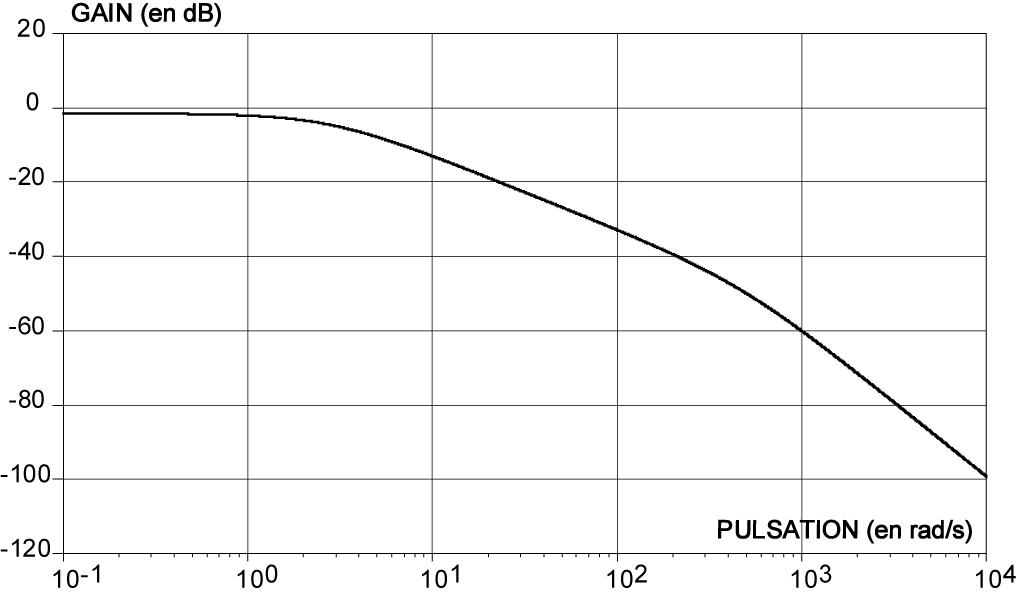
\includegraphics[width=\linewidth]{68_02}
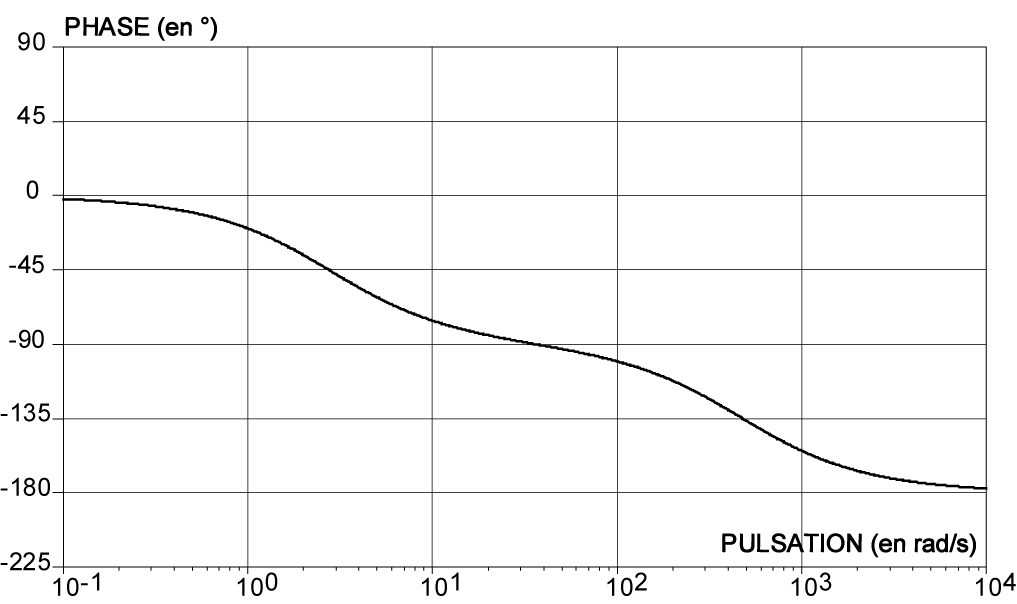
\includegraphics[width=\linewidth]{68_03}
\end{center}
\fi

\question{Le système étudié est-il stable théoriquement ? Justifier vos réponses.}
\ifprof
\else 
\fi

\question{Etudier l’aptitude du système sans correction à respecter les critères de précision. Vous déterminerez
notamment les expressions littérales de l’erreur statique en poursuite pour une consigne de vitesse de la
plate-forme $V_c (t)$ en échelon d’amplitude $V_{\text{CO}}$ : $V_C(t) = V_{\text{CO}}  u(t)$ (avec $u(t)$ l’échelon unitaire) et de l’influence en régulation d’une perturbation $C_{\text{equ}} (t)$ en échelon d’amplitude $C_0$, sur la vitesse réelle $V (t)$ de la plate-forme en régime permanent.}
\ifprof
\else 
\fi

\textbf{Etude des performances avec un correcteur de fonction de transfert : $C(p)=\dfrac{K_I}{p}$}

\question{Indiquer quelle est la nature de la correction effectuée par ce correcteur (ou désignation du correcteur) ?
Indiquer pour quelle(s) raison(s) principale(s) ce correcteur a été choisi. Valider ce choix vis à vis du cahier
des charges. Sans calcul, donner l’influence de ce correcteur sur les autres performances attendues.}
\ifprof
\else 
\fi

Reprenons le diagramme de Bode précédent.

\question{Compléter le document-réponse en traçant les diagrammes de Bode du
correcteur avec $K_I = \SI{1}{s^{-1}}$ . Déterminer alors la valeur de $K_I$ maximale notée $K_{\text{I max}}$ permettant de respecter les marges de stabilité énoncées dans le cahier des charges.}
\ifprof
\else 
\fi

\ifprof
\else
Afin d’évaluer analytiquement le temps de réponse à 5\%, Il est proposé d’adopter une modélisation simplifiée du
comportement du moteur en conservant uniquement le mode associé au pôle << dominant >>. On donne $T_{5\% \text{mini}}\cdot \omega_0 = 3$ avec $\omega_0$ la pulsation propre non amortie d’un système fondamental du second ordre.
\fi

\question{En analysant les valeurs numériques des pôles de la fonction de transfert du moteur en poursuite $H_U( p)$,
préciser quel est le pôle dominant et proposer alors un modèle simplifié de la fonction de transfert $H_U ( p)$.
Déterminer alors la valeur numérique de $K_I$ notée $K_{I\SI{5}{\%}}$ minimisant le temps de réponse à 5\% pour une
entrée échelon en poursuite. Calculer alors la valeur approchée du temps de réponse à 5\% minimale $T_{5\% \text{mini}}$ et comparer la au cahier des charges.}
\ifprof
\else 
\fi

\textbf{Etude des performances avec un correcteur proportionnel intégral : $C(p)=K_P \left( 1+\dfrac{1}{T_i p}\right)$}

\ifprof
\else
Le correcteur est remplacé par un correcteur proportionnel intégral. Des réponses temporelles du système corrigé sont
tracées avec :
\begin{itemize}
\item une consigne de vitesse unitaire de la plate-forme $V_c (t)= u(t)$ (avec $u(t)$ l’échelon unitaire) ;
\item une perturbation sous la forme d’un échelon unitaire retardé de 5 secondes $C_{\text{equ}} (t) = u(t - 5)$ ;
\item un gain du correcteur $K_P= 1$ ;
\item différentes valeurs de $T_I$.
\end{itemize}

\begin{center}
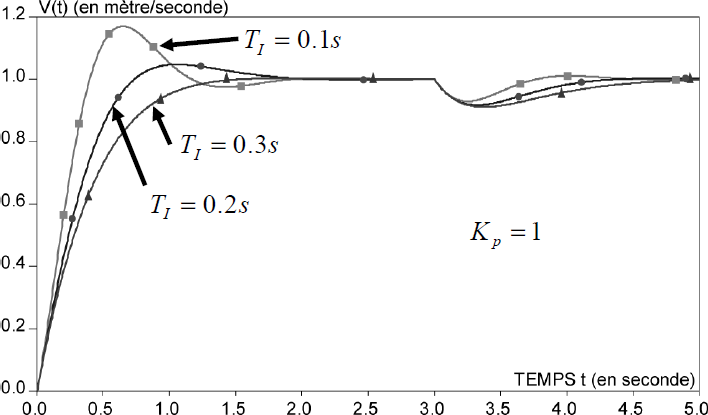
\includegraphics[width=\linewidth]{68_04}
\end{center}
\fi

\question{Parmi les différentes valeurs de $T_I$ , choisir celle qui assure le temps de réponse à 5\% le plus faible. Vous
ferez apparaître ce temps de réponse sur la figure.}
\ifprof
\else 
\fi


\ifprof
\else 
La valeur de $T_I$ déterminée à la question précédente est retenue pour le réglage du correcteur proportionnel intégral.
Il s’agit alors de choisir le gain du correcteur $K_p$ à partir des simulations proposées.

\begin{center}
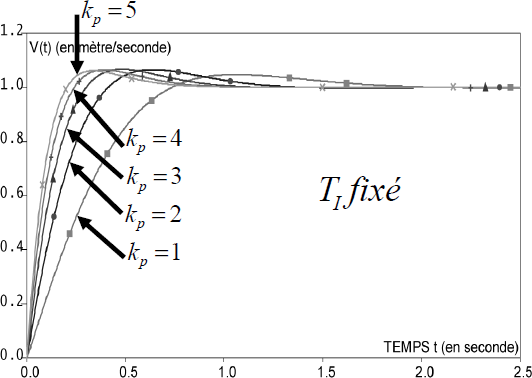
\includegraphics[width=\linewidth]{68_05}
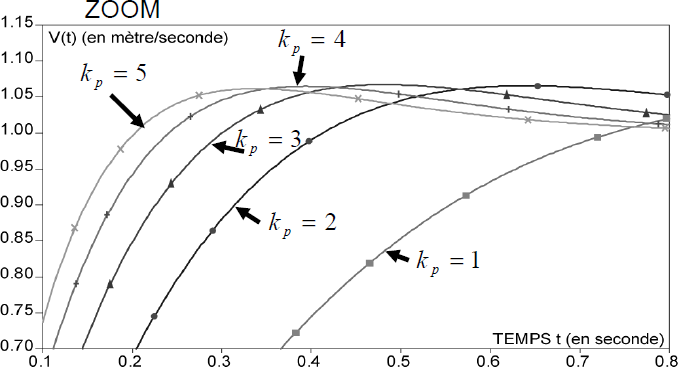
\includegraphics[width=\linewidth]{68_06}
\end{center}
\fi

\question{Parmi les différentes valeurs de $K_p$ , choisir la valeur qui assure un temps de réponse à 5\% au plus près de
la valeur fournie dans le cahier des charges.}
\ifprof
\else 
\fi

\ifprof
\else 

Avec le couple de valeurs ($T_I$ et $K_p$) obtenu, la réponse fréquentielle du système en boucle ouverte a été tracée.
\begin{center}
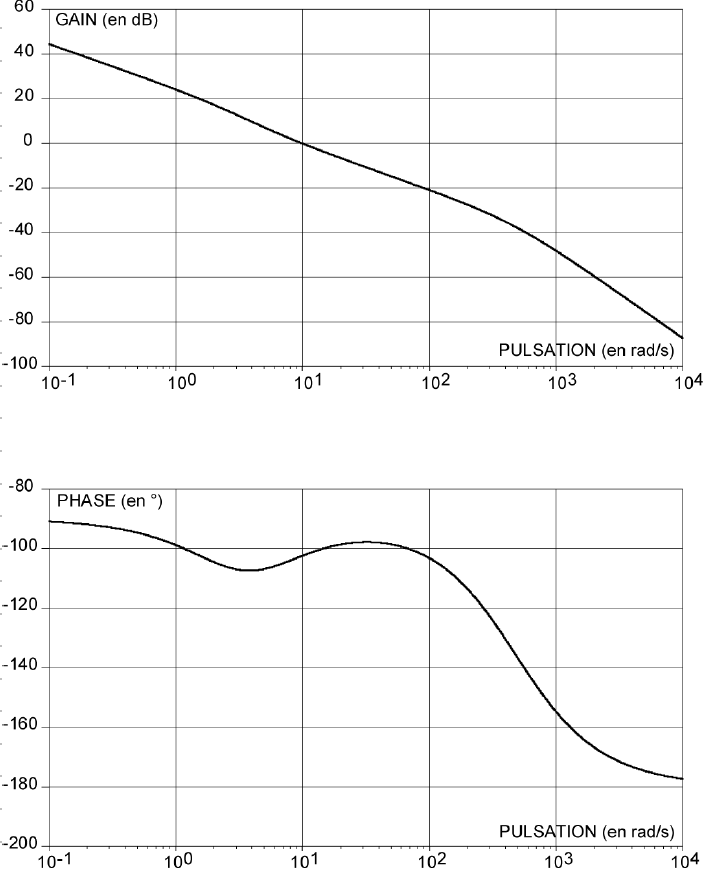
\includegraphics[width=\linewidth]{68_07}
\end{center}
\fi


\question{Conclure quant à la capacité de ce correcteur à respecter tous les critères du cahier des charges.}
\ifprof
\else 
\fi


\ifprof
\else

\noindent\footnotesize
 \fbox{\parbox{.9\linewidth}{
Éléments de corrigé : 
\begin{enumerate}
\item .
\end{enumerate}}}
\normalsize

\begin{flushright}
\footnotesize{Corrigé  voir \ref{C2:04:68}.}
\end{flushright}%
\fi